\documentclass[11pt]{article}
\usepackage[textwidth=18.0cm, textheight=23.0cm, top=2.0cm]{geometry}
\usepackage{pst-all}
\usepackage{amssymb}
\usepackage{tikz}
\usepackage{underscore}\begin{document}
\pagestyle{empty}


ClassName: \underline{\textbf{Class_05.2bp-6}}
\par
BinSize: \underline{\textbf{100 × 100}}
\par
ReduceSize: \underline{\textbf{100 × 100}}
\par
TypeNum: \underline{\textbf{20}}
\par
Num: \underline{\textbf{20}}
\par
OutS: \underline{\textbf{60000}}
\par
InS: \underline{\textbf{42656}}
\par
Rate: \underline{\textbf{0.711}}
\par
UB: \underline{\textbf{6}}
\par
LB0: \underline{\textbf{6}}
\par
LB: \underline{\textbf{6}}
\par
LBWithCut: \underline{\textbf{6}}
\par
NodeCut: \underline{\textbf{0}}
\par
ExtendedNodeCnt: \underline{\textbf{1}}
\par
GenNodeCnt: \underline{\textbf{1}}
\par
PrimalNode: \underline{\textbf{0}}
\par
ColumnCount: \underline{\textbf{6}}
\par
TotalCutCount: \underline{\textbf{0}}
\par
RootCutCount: \underline{\textbf{0}}
\par
LPSolverCnt: \underline{\textbf{1}}
\par
PricingSolverCnt: \underline{\textbf{0}}
\par
BranchAndBoundNum: \underline{\textbf{1}}
\par
isOpt: \underline{\textbf{true}}
\par
TimeOnInitSolution: \underline{\textbf{600.000 s}}
\par
TimeOnPrimal: \underline{\textbf{0.000 s}}
\par
TimeOnPricing: \underline{\textbf{0.000 s}}
\par
TimeOnRmp: \underline{\textbf{0.046 s}}
\par
TotalTime: \underline{\textbf{600.328 s}}
\par
\newpage


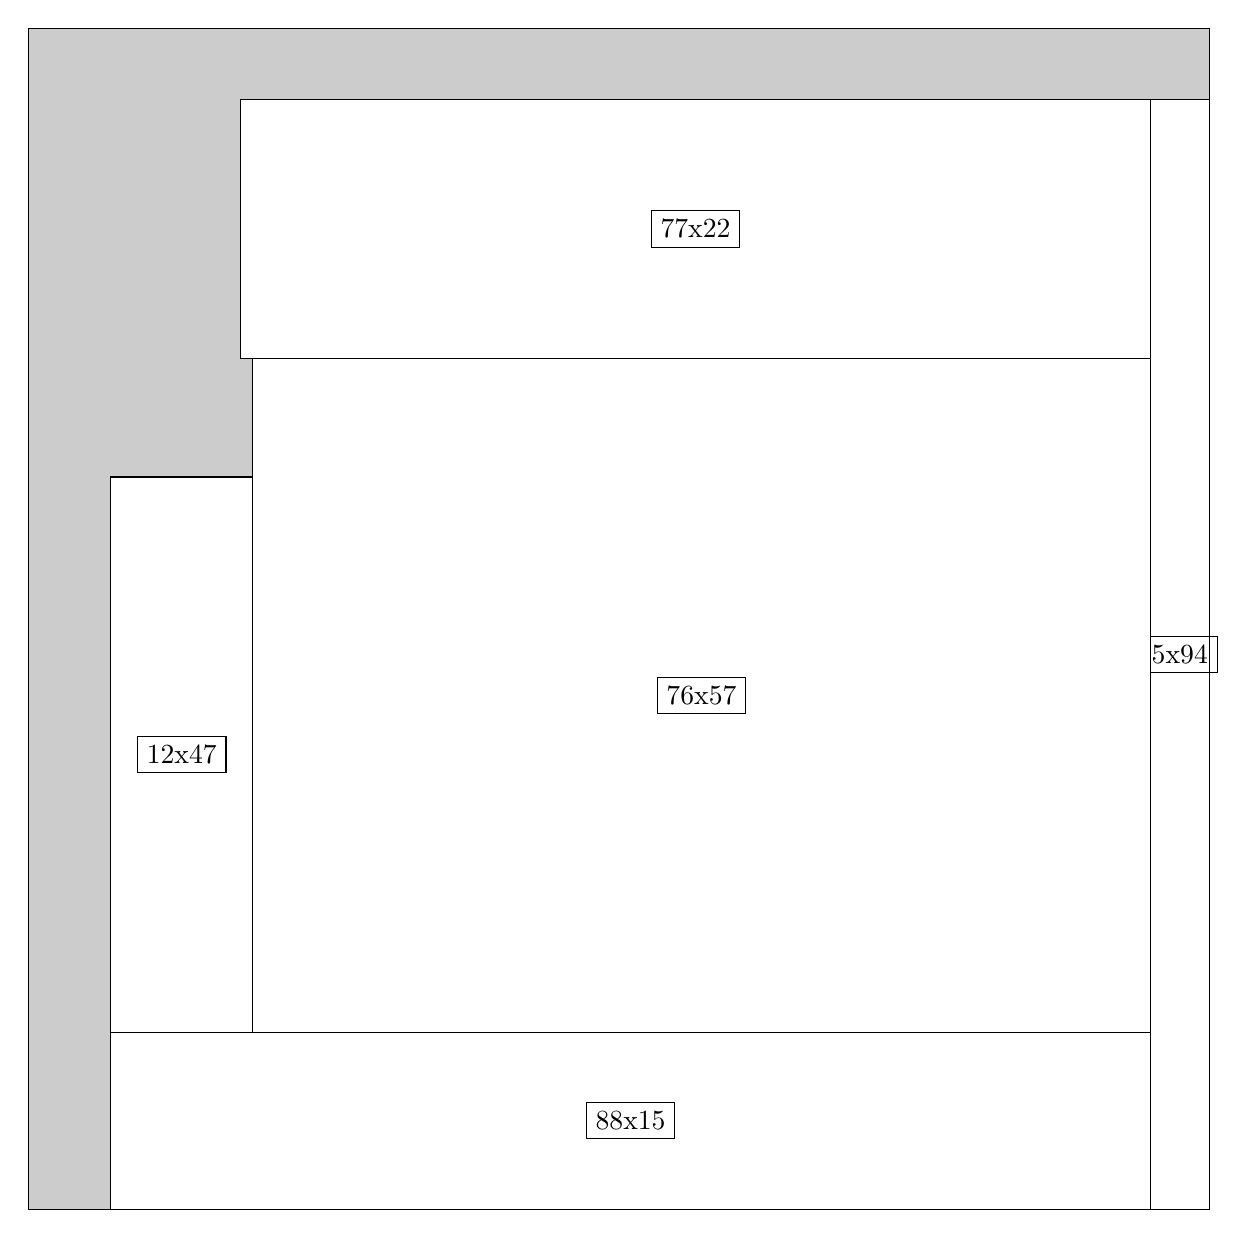
\begin{tikzpicture}[shorten >=1pt,scale=1.0,every node/.style={scale=1.0},->]
\tikzstyle{vertex}=[circle,fill=black!25,minimum size=14pt,inner sep=0pt]
\filldraw[fill=gray!40!white, draw=black] (0,0) rectangle (15.0,15.0);
\foreach \name/\x/\y/\w/\h in {5x94/14.25/0.0/0.75/14.1,88x15/1.05/0.0/13.2/2.25,76x57/2.85/2.25/11.4/8.549999999999999,12x47/1.05/2.25/1.7999999999999998/7.05,77x22/2.6999999999999997/10.799999999999999/11.549999999999999/3.3}
\filldraw[fill=white!40!white, draw=black] (\x,\y) rectangle node[draw] (\name) {\name} ++(\w,\h);
\end{tikzpicture}


w =5 , h =94 , x =95 , y =0 , v =470
\par
w =88 , h =15 , x =7 , y =0 , v =1320
\par
w =76 , h =57 , x =19 , y =15 , v =4332
\par
w =12 , h =47 , x =7 , y =15 , v =564
\par
w =77 , h =22 , x =18 , y =72 , v =1694
\par
\newpage


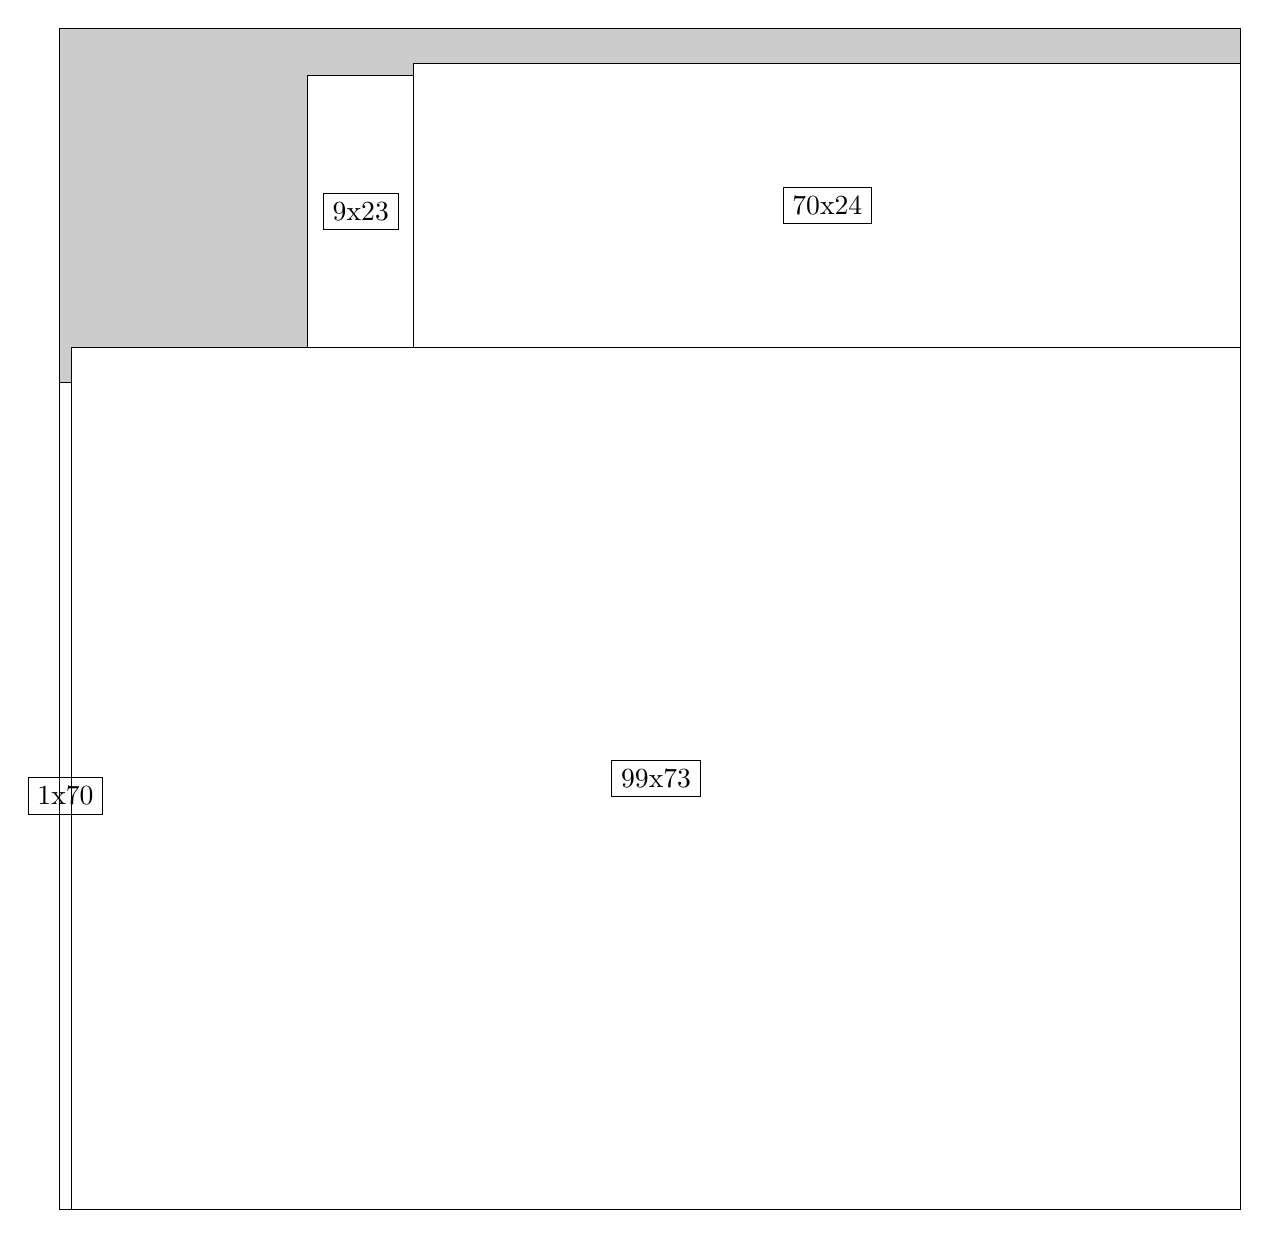
\begin{tikzpicture}[shorten >=1pt,scale=1.0,every node/.style={scale=1.0},->]
\tikzstyle{vertex}=[circle,fill=black!25,minimum size=14pt,inner sep=0pt]
\filldraw[fill=gray!40!white, draw=black] (0,0) rectangle (15.0,15.0);
\foreach \name/\x/\y/\w/\h in {99x73/0.15/0.0/14.85/10.95,1x70/0.0/0.0/0.15/10.5,70x24/4.5/10.95/10.5/3.5999999999999996,9x23/3.15/10.95/1.3499999999999999/3.4499999999999997}
\filldraw[fill=white!40!white, draw=black] (\x,\y) rectangle node[draw] (\name) {\name} ++(\w,\h);
\end{tikzpicture}


w =99 , h =73 , x =1 , y =0 , v =7227
\par
w =1 , h =70 , x =0 , y =0 , v =70
\par
w =70 , h =24 , x =30 , y =73 , v =1680
\par
w =9 , h =23 , x =21 , y =73 , v =207
\par
\newpage


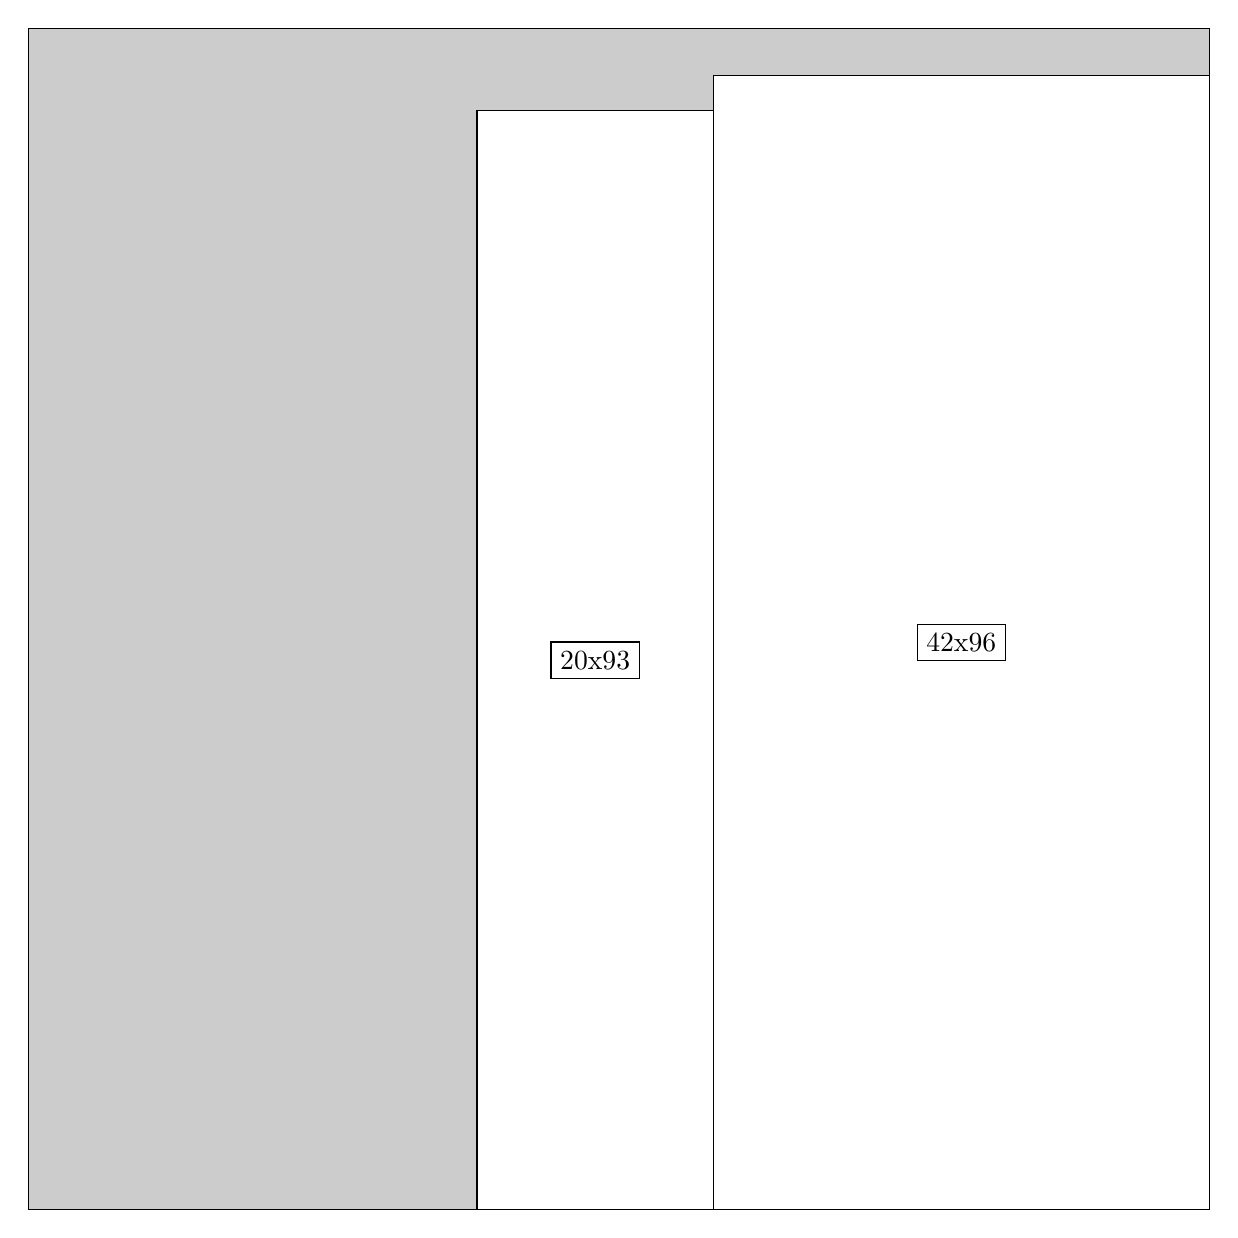
\begin{tikzpicture}[shorten >=1pt,scale=1.0,every node/.style={scale=1.0},->]
\tikzstyle{vertex}=[circle,fill=black!25,minimum size=14pt,inner sep=0pt]
\filldraw[fill=gray!40!white, draw=black] (0,0) rectangle (15.0,15.0);
\foreach \name/\x/\y/\w/\h in {42x96/8.7/0.0/6.3/14.399999999999999,20x93/5.7/0.0/3.0/13.95}
\filldraw[fill=white!40!white, draw=black] (\x,\y) rectangle node[draw] (\name) {\name} ++(\w,\h);
\end{tikzpicture}


w =42 , h =96 , x =58 , y =0 , v =4032
\par
w =20 , h =93 , x =38 , y =0 , v =1860
\par
\newpage


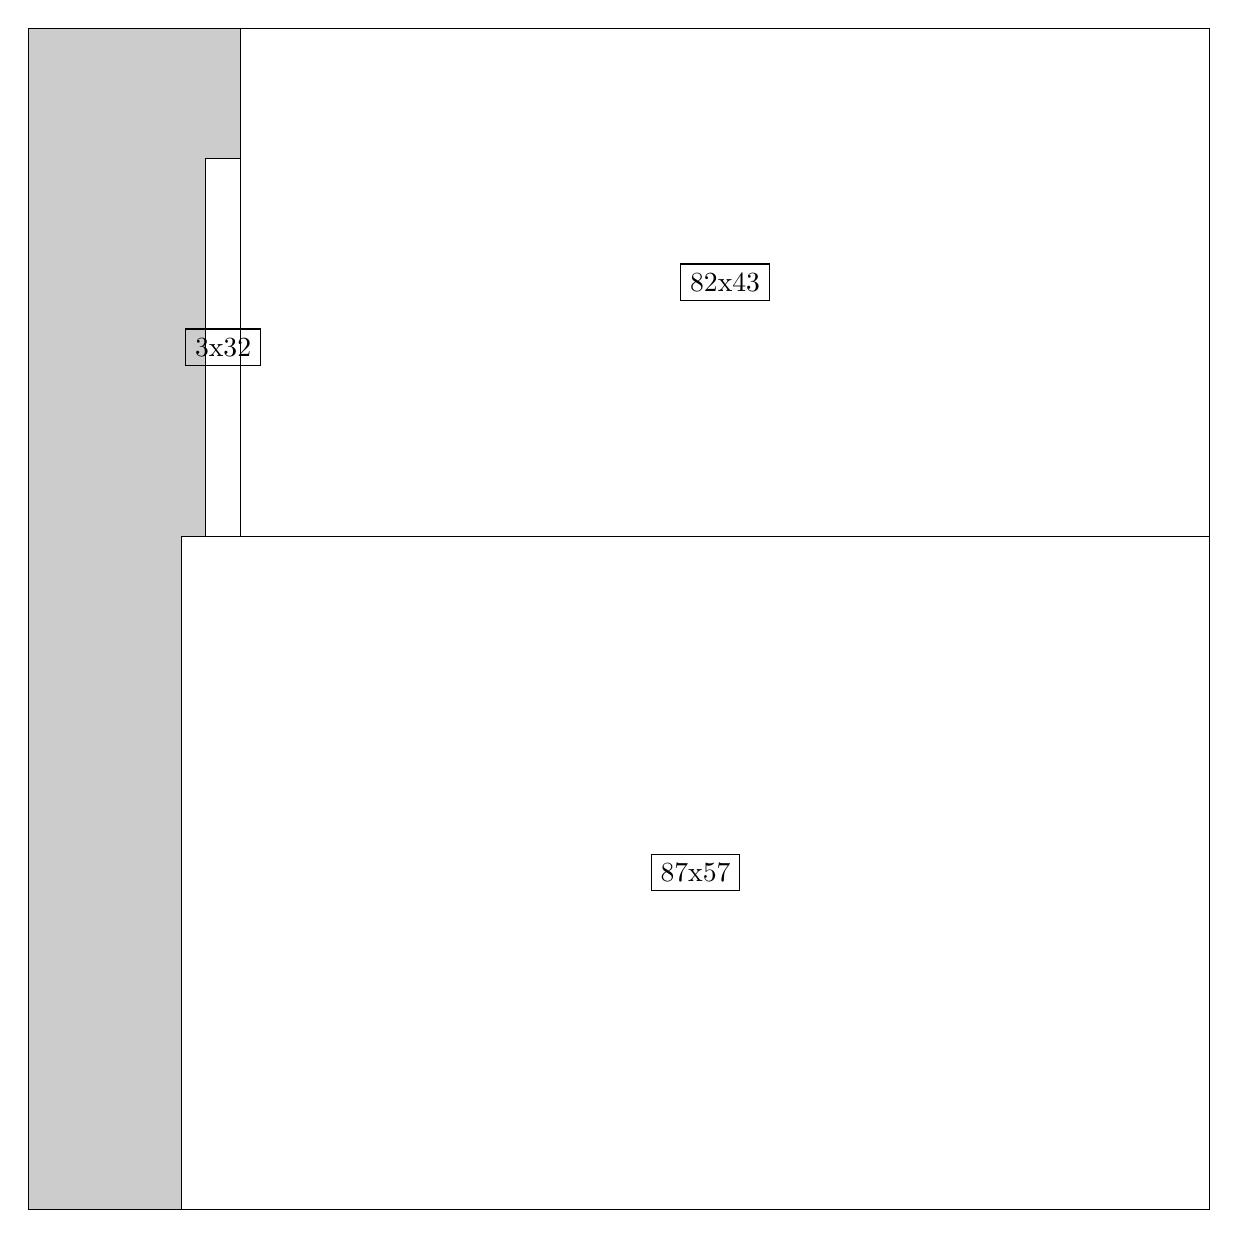
\begin{tikzpicture}[shorten >=1pt,scale=1.0,every node/.style={scale=1.0},->]
\tikzstyle{vertex}=[circle,fill=black!25,minimum size=14pt,inner sep=0pt]
\filldraw[fill=gray!40!white, draw=black] (0,0) rectangle (15.0,15.0);
\foreach \name/\x/\y/\w/\h in {87x57/1.95/0.0/13.049999999999999/8.549999999999999,82x43/2.6999999999999997/8.549999999999999/12.299999999999999/6.45,3x32/2.25/8.549999999999999/0.44999999999999996/4.8}
\filldraw[fill=white!40!white, draw=black] (\x,\y) rectangle node[draw] (\name) {\name} ++(\w,\h);
\end{tikzpicture}


w =87 , h =57 , x =13 , y =0 , v =4959
\par
w =82 , h =43 , x =18 , y =57 , v =3526
\par
w =3 , h =32 , x =15 , y =57 , v =96
\par
\newpage


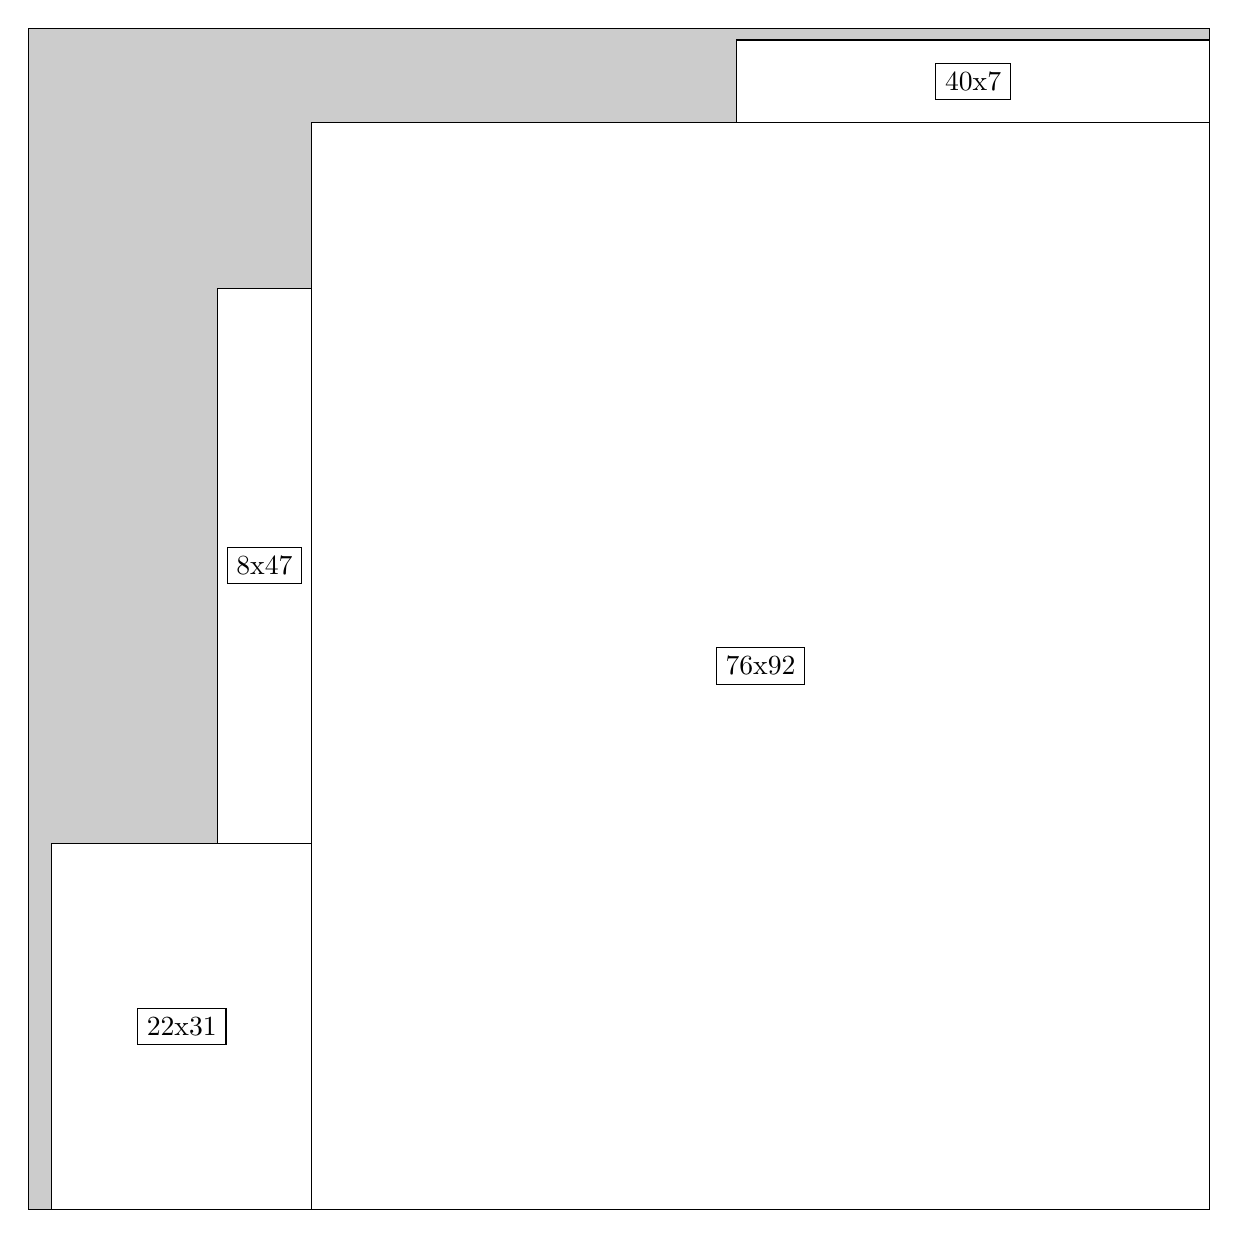
\begin{tikzpicture}[shorten >=1pt,scale=1.0,every node/.style={scale=1.0},->]
\tikzstyle{vertex}=[circle,fill=black!25,minimum size=14pt,inner sep=0pt]
\filldraw[fill=gray!40!white, draw=black] (0,0) rectangle (15.0,15.0);
\foreach \name/\x/\y/\w/\h in {76x92/3.5999999999999996/0.0/11.4/13.799999999999999,22x31/0.3/0.0/3.3/4.6499999999999995,8x47/2.4/4.6499999999999995/1.2/7.05,40x7/9.0/13.799999999999999/6.0/1.05}
\filldraw[fill=white!40!white, draw=black] (\x,\y) rectangle node[draw] (\name) {\name} ++(\w,\h);
\end{tikzpicture}


w =76 , h =92 , x =24 , y =0 , v =6992
\par
w =22 , h =31 , x =2 , y =0 , v =682
\par
w =8 , h =47 , x =16 , y =31 , v =376
\par
w =40 , h =7 , x =60 , y =92 , v =280
\par
\newpage


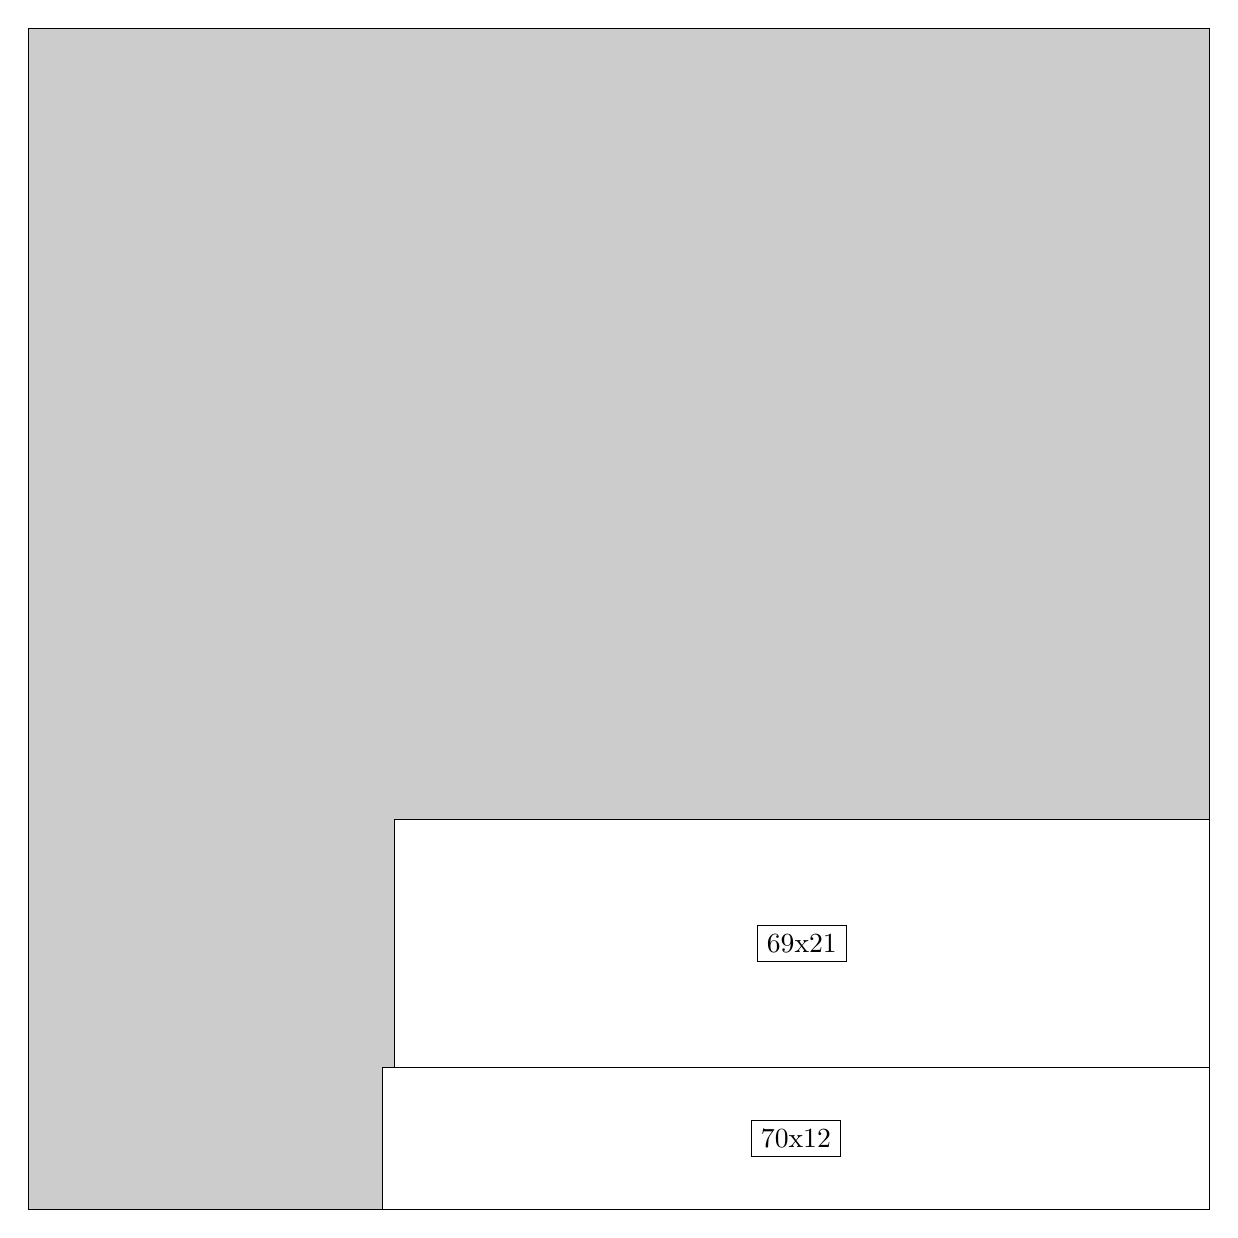
\begin{tikzpicture}[shorten >=1pt,scale=1.0,every node/.style={scale=1.0},->]
\tikzstyle{vertex}=[circle,fill=black!25,minimum size=14pt,inner sep=0pt]
\filldraw[fill=gray!40!white, draw=black] (0,0) rectangle (15.0,15.0);
\foreach \name/\x/\y/\w/\h in {70x12/4.5/0.0/10.5/1.7999999999999998,69x21/4.6499999999999995/1.7999999999999998/10.35/3.15}
\filldraw[fill=white!40!white, draw=black] (\x,\y) rectangle node[draw] (\name) {\name} ++(\w,\h);
\end{tikzpicture}


w =70 , h =12 , x =30 , y =0 , v =840
\par
w =69 , h =21 , x =31 , y =12 , v =1449
\par
\newpage


\end{document}